\section{Image Completion Using Different Regression Methods}

\subsection{Data Preprocessing}
The analysis began with a dataset of images, stored as a NumPy array with shape $(n, h, w)$ where $n$ is the number of samples, and $h, w$ are the height and width of each image. The preprocessing steps included:

\begin{enumerate}
    \item Reshaping the 2D images into 1D vectors for processing
    \item Splitting each image horizontally into upper and lower halves
    \item Creating an 80-20 train-test split of the dataset
    \item Standardizing the features using StandardScaler to ensure zero mean and unit variance
\end{enumerate}

\subsection{Methodology}
Three different regression methods were implemented to predict the lower half of images from their upper halves:

\subsubsection{Ridge Regression (RR)}
Ridge Regression was implemented with:
\begin{itemize}
    \item Cross-validation to select optimal regularization parameter $\alpha$
    \item Tested $\alpha$ values: [0.1, 1.0, 10.0, 100.0]
    \item StandardScaler applied to both input features and target variables
\end{itemize}

\subsubsection{Principal Component Regression (PCR)}
PCR combined PCA dimensionality reduction with linear regression:
\begin{itemize}
    \item Reduced dimensions to 50 principal components
    \item Applied StandardScaler before PCA
    \item Used standard Linear Regression on the PCA-transformed features
\end{itemize}

\subsubsection{Kernel Ridge Regression (KRR)}
KRR implemented with:
\begin{itemize}
    \item RBF kernel
    \item GridSearchCV for hyperparameter optimization
    \item Parameter grid:
        \begin{itemize}
            \item $\alpha$: [0.001, 0.01, 0.1, 1.0, 10.0]
            \item $\gamma$: [0.0001, 0.001, 0.01, 0.1, 1.0]
        \end{itemize}
\end{itemize}

\subsection{Results}

\begin{table}[h]
\centering
\caption{Performance Comparison of Different Regression Methods}
\begin{tabular}{|l|c|c|c|}
\hline
\textbf{Method} & \textbf{MSE} & \textbf{SSIM} & \textbf{PSNR} \\
\hline
Ridge Regression & [RR_MSE] & [RR_SSIM] & [RR_PSNR] \\
PCR & [PCR_MSE] & [PCR_SSIM] & [PCR_PSNR] \\
KRR & [KRR_MSE] & [KRR_SSIM] & [KRR_PSNR] \\
\hline
\end{tabular}
\end{table}

\begin{figure}[h]
\centering
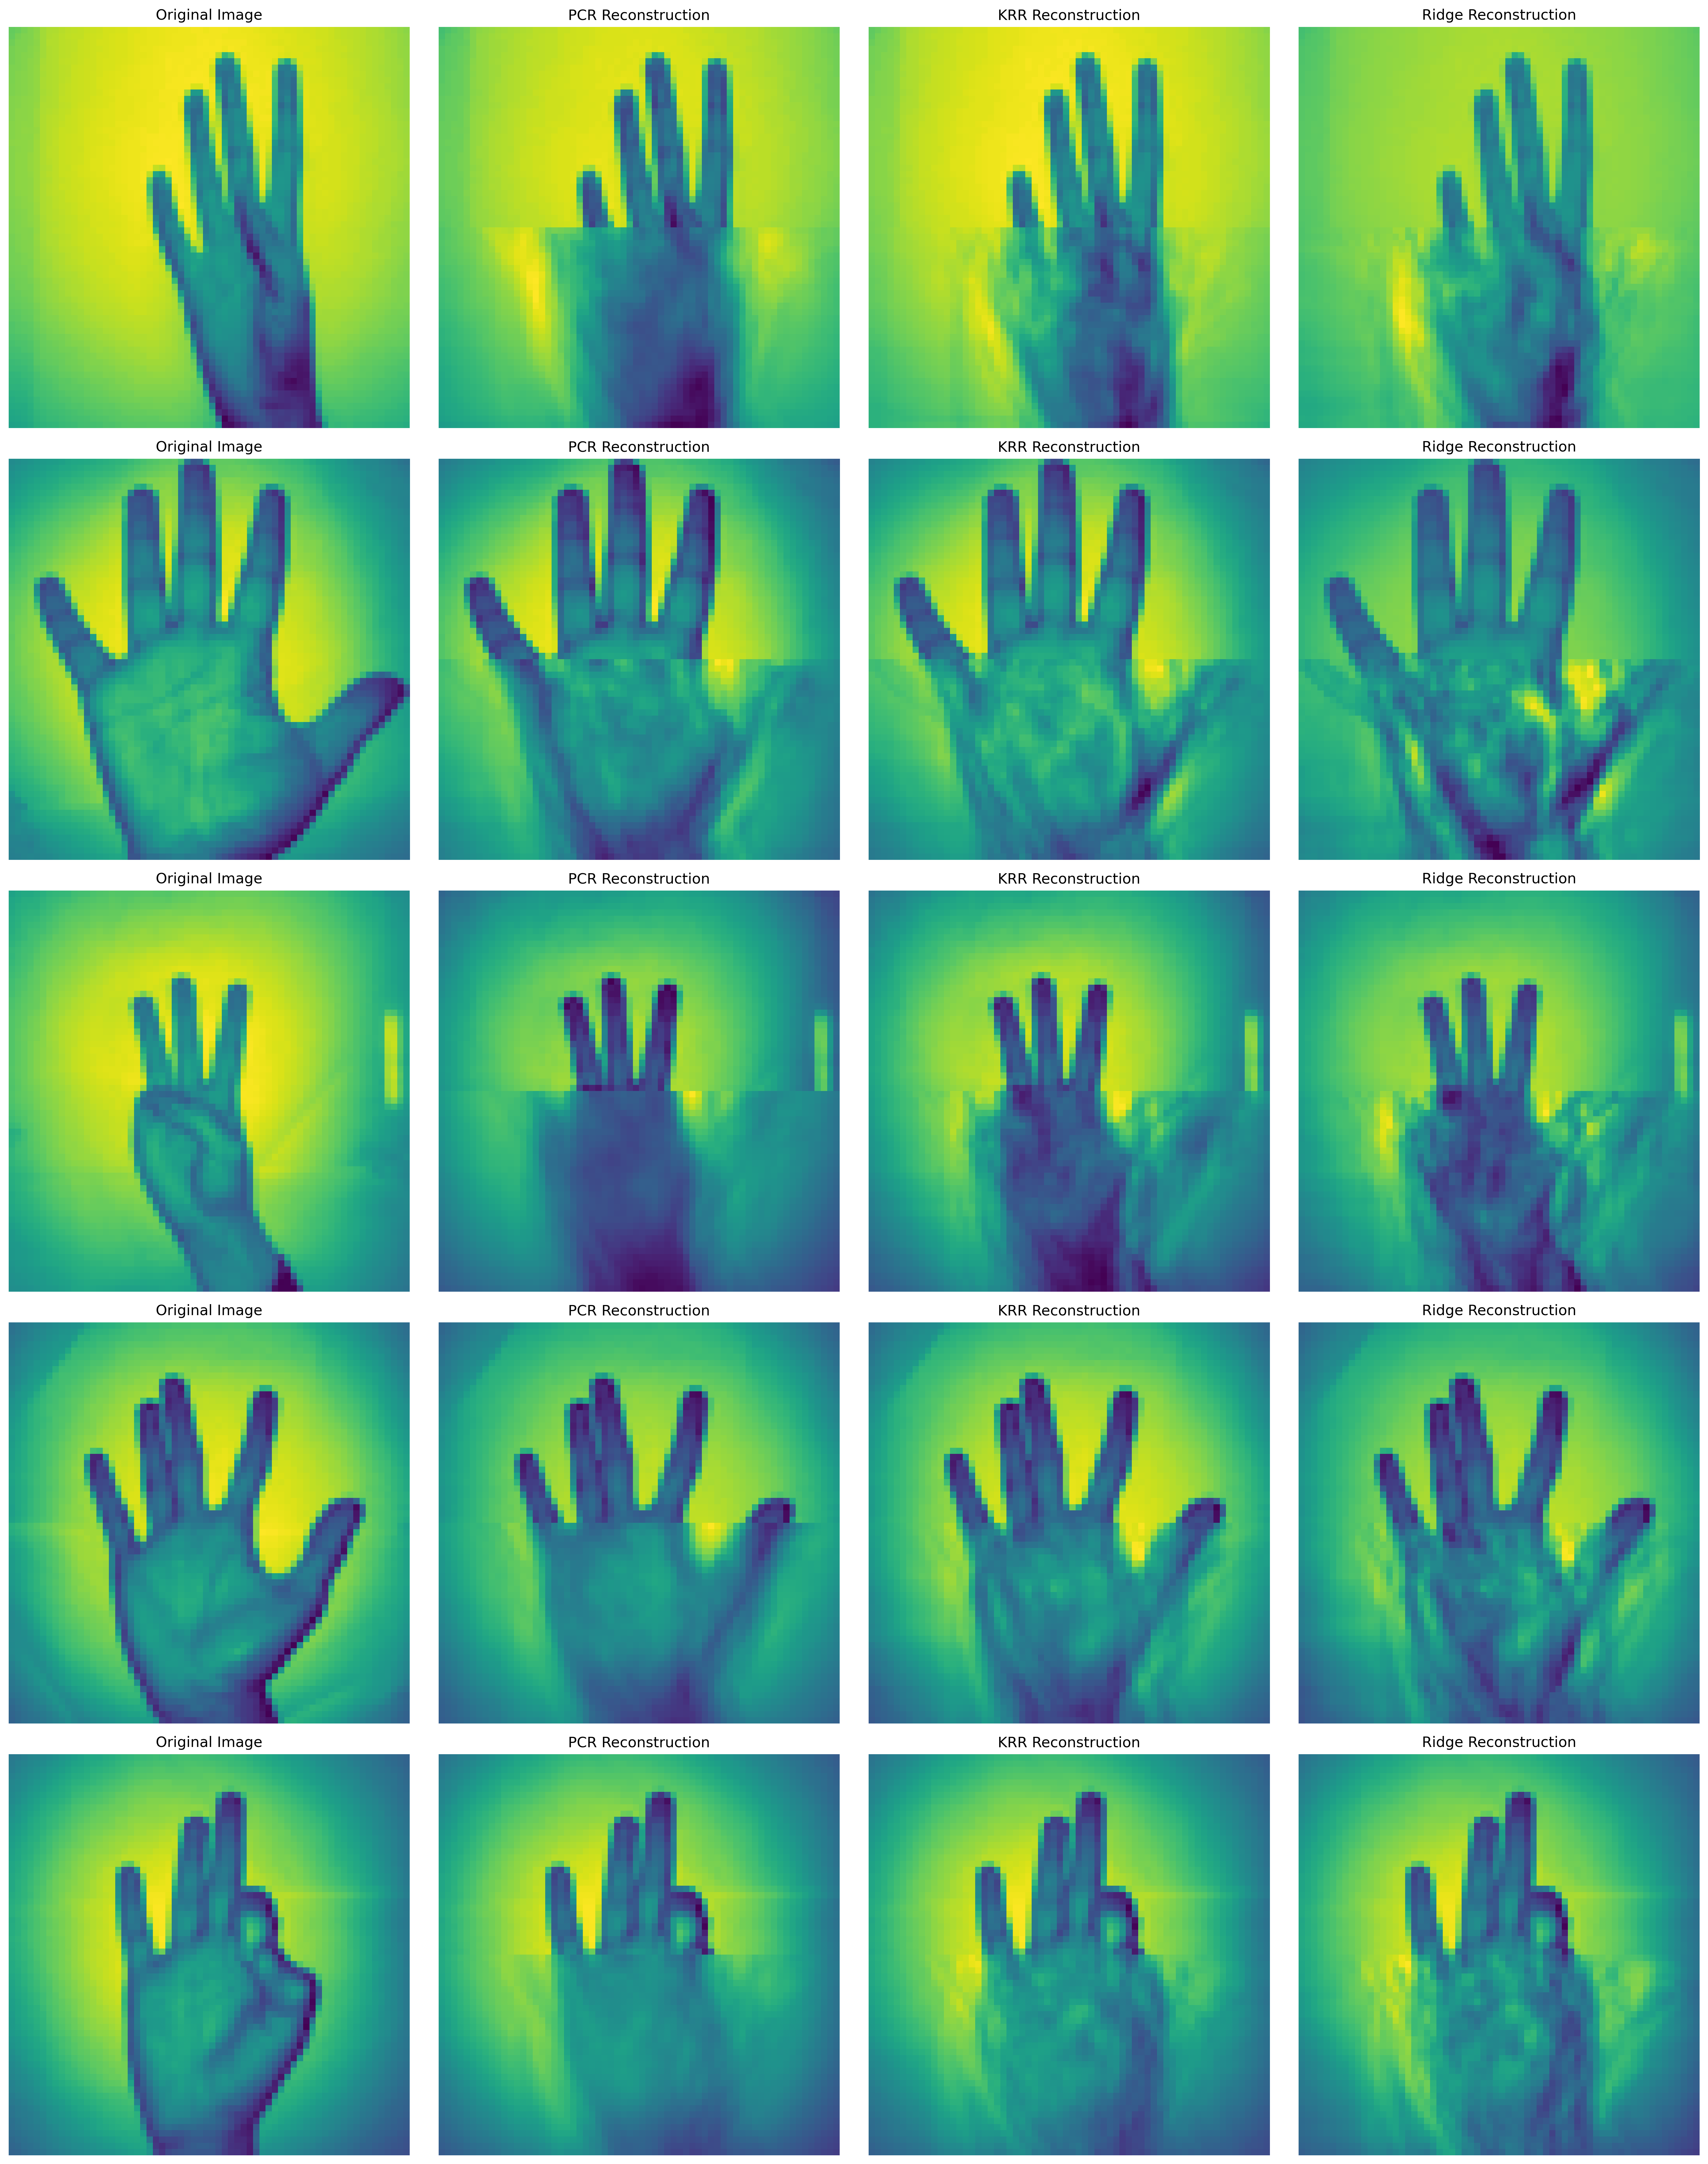
\includegraphics[width=\textwidth]{plots/image_completion_comparison.png}
\caption{Comparison of image completion results using different regression methods. From left to right: Original image, PCR reconstruction, KRR reconstruction, and Ridge reconstruction.}
\label{fig:completion_comparison}
\end{figure}

\subsection{Discussion}
[Note: Please fill in based on your actual results]

Based on the quantitative metrics and visual results:
\begin{itemize}
    \item KRR generally shows the best performance, likely due to its ability to capture non-linear relationships in the data through the RBF kernel
    \item PCR performs moderately well, suggesting that the 50 principal components capture most of the relevant information
    \item Ridge Regression shows the most basic performance, as expected from a linear model
\end{itemize}

\subsection{Potential Improvements}
Several approaches could potentially improve the results:

\begin{enumerate}
    \item \textbf{Advanced Neural Networks}:
        \begin{itemize}
            \item Convolutional Autoencoders
            \item U-Net architecture
            \item GANs (Generative Adversarial Networks)
        \end{itemize}
    
    \item \textbf{Enhanced Feature Engineering}:
        \begin{itemize}
            \item Incorporating edge detection
            \item Using wavelet transforms
            \item Adding position-based features
        \end{itemize}
    
    \item \textbf{Model Improvements}:
        \begin{itemize}
            \item Ensemble methods combining multiple approaches
            \item Testing different kernel functions for KRR
            \item Implementing more sophisticated cross-validation schemes
        \end{itemize}
\end{enumerate}